\chapter{Laboratorio 2}
In questa esperienza di laboratorio, si sono analizzati tre circuiti che svolgono la funzione di raddrizzatori grazie alla presenza di uno o più diodi (\Fig\ref{fig:diodo}). In particolare, si è utilizzato il diodo 1N4148 \url{https://www.diodes.com/assets/Datasheets/ds12019.pdf}.
\begin{figure}[h]
	\centering
	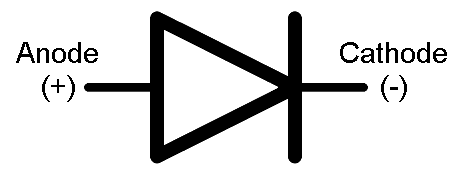
\includegraphics[width=0.3\linewidth]{./ImageFiles/Laboratorio 2/diodo_1}
	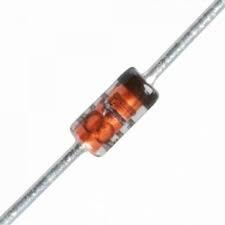
\includegraphics[width=0.2\linewidth]{./ImageFiles/Laboratorio 2/diodo_4}
	\caption{Rappresentazione simbolica di un diodo e foto del diodo 1N4148.}
	\label{fig:diodo}
\end{figure}
Il diodo è un dipolo che permette di realizzare circuiti raddrizzatori grazie al suo comportamento che differisce in base alle condizioni del circuito in cui è inserito. In particolare, se la tensione all'anodo è maggiore di una certa tensione di soglia (tipicamente considerata pari a \SI{0.7}{\volt}) rispetto alla tensione a cui si trova il catodo, il diodo permette il passaggio di corrente dall'anodo al catodo. Al contrario, non è consentito il passaggio di corrente dal catodo all'anodo. Più precisamente, la relazione corrente-tensione è descritta dalla seguente legge esponenziale:
\begin{equation}
	I_D=I_S[e^{\frac{V_D}{V_T}}-1],
\end{equation}
dove $I\sub{D}$ è la corrente nel diodo (con verso positivo dall'anodo al catodo), $I\sub{S}$ è la corrente inversa, $V\sub{D}$ è la differenza di tensione tra anodo e catodo mentre $V\sub{T}$ è la tensione termica. In figura \ref{fig:diodo_caratteristica} è rappresentata la caratteristica corrente-tensione dei due modelli del diodo: quello ideale e quello reale. In particolare, si definisce regione di funzionamento diretta quando il diodo è acceso e permette il passaggio di corrente da anodo a catodo ($V_{D}>0$) e regione inversa quando il diodo è spento e impedisce il passaggio di corrente (o più precisamente, la corrente è pari a $-I\sub{S}$).
\begin{figure}[h]
	\centering
	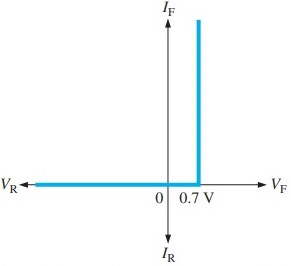
\includegraphics[width=0.3\linewidth]{./ImageFiles/Laboratorio 2/diodo_2}
	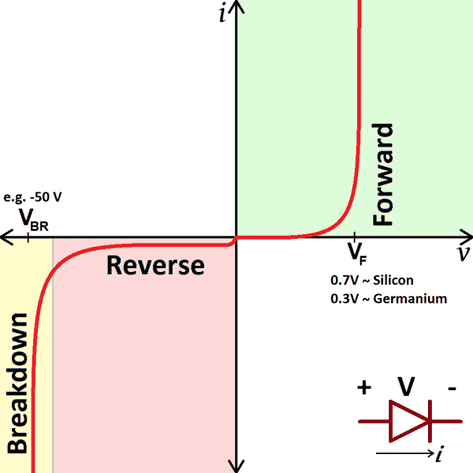
\includegraphics[width=0.3\linewidth]{./ImageFiles/Laboratorio 2/diodo_3}
	\caption{Caratteristica corrente-tensione del modello ideale (sinistra) e reale (destra) di un diodo.}
	\label{fig:diodo_caratteristica}
\end{figure}

Il primo circuito realizzato è un semplice raddrizzatore a singola semionda che utilizza un unico diodo e una resistenza. Lo schema del circuito è riportato in figura \ref{xxx}.
\begin{figure}[h]
	\centering
	%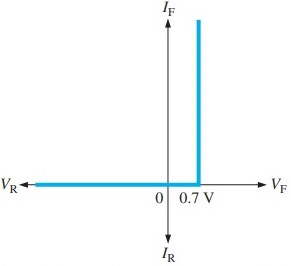
\includegraphics[width=0.3\linewidth]{./ImageFiles/Laboratorio 2/diodo_2}
	\caption{Schema circuitale del raddrizzatore a singola semionda.}
	%\label{fig:diodo_caratteristica}
\end{figure}\todo{inserire schema e foto del circuito. indicare con D i diodi, R resistenze}
Considerando il modello ideale del diodo, è possibile analizzare il comportamento del circuito quando in ingresso è applicata una tensione sinusoidale. Considerando una tensione di soglia del diodo pari a \SI{0.7}{\volt} si ha che:
\begin{itemize}
	\item se $v_{in}>\SI{0.7}{\volt}$ allora $v\sub{out}=\SI{0}{\volt}$, poiché nel circuito non scorre corrente, nemmeno nella resistenza R che quindi mantiene a massa il nodo $v\sub{out}$;
	\item se $v_{in} >= \SI{0.7}{\volt}$ il diodo $D$ si accende; quindi sul nodo $v\sub{out}$ avremo $v_{out}=v_{in}-\SI{0.7}{\volt}$.
\end{itemize}
Per analizzare il comportamento del circuito si sono effettuate delle misure tramite l'oscilloscopio sui nodi$ v\sub{in}$ e $v\sub{out}$, applicando in ingresso sul nodo $v\sub{in}$ una sinusoide di ampiezza picco-picco pari a \SI{2}{\volt} e variando il valore della resistenza e della frequenza del segnale in ingresso. Nella tabella \ref{tab:valori_componenti_1} sono indicati i valori nominali e misurati delle resistenze utilizzate. \`E stata inoltre misurata la tensione di soglia del diodo utilizzato, che è risultata essere pari a \SI{0.618}{\volt}.

\def\arraystretch{1.3}
\begin{table}[h]
	\centering
	\begin{tabular}{|c|c|c|}
		\hline
		Componente	& Valore Nominale & Valore Misurato \\ \hline
		R\sub{1}          & \SI{0}{\kilo\ohm} &     \SI{0}{\kilo\ohm}  \\ \hline
		R\sub{2}          & \SI{0}{\kilo\ohm} &     \SI{0}{\kilo\ohm} \\ \hline
		R\sub{3}          & \SI{0}{\kilo\ohm} &     \SI{0}{\kilo\ohm} \\ \hline
		R\sub{4}          & \SI{0}{\kilo\ohm} &     \SI{0}{\kilo\ohm} \\ \hline
	\end{tabular}
	\caption{Valori nominali e misurati delle resistenze utilizzate nel circuito.}
	\label{tab:valori_componenti_1}
\end{table}
Nella figura \ref{fig} sono rappresentate le differenti misure effettuate a frequenza fissa pari a xxx, variando la resistenza utilizzata.
\todo{inserire immagini R diverse e stessa frequenza}
Come si può osservare, in un diodo reale c'è una dipendenza della tensione di soglia dalla corrente che lo attraversa: infatti, aumentando la resistenza diminuisce la corrente che circola nel circuito e quindi anche la tensione di soglia. Al contrario, diminuendo il valore della resistenza R aumenta la corrente che circola nel circuito e quindi aumenta la tensione di soglia.
Successivamente si è analizzato il comportamento in frequenza del circuito, variando la frequenza della sinusoide in ingresso. Per le misure, si sono scelte le frequenze di \SI{1}{\kilo\hertz}, \SI{10}{\kilo\hertz}, \SI{100}{\kilo\hertz} e \SI{1}{\mega\hertz} (\Fig\ref{fig}).
\todo{inserire immagini con frequenze diverse}
Osservando le acquisizioni si nota che aumentando la frequenza il segnale in uscita presenta una semionda distorta. In particolare, si può notare che il diodo riesce a seguire abbastanza correttamente il fronte di salita del segnale in ingresso (il diodo in questa fase si accende). Tuttavia, il diodo non è sufficientemente veloce nella fase di spegnimento, producendo un'onda che lentamente ritorna a zero \todo{non so come dirla meglio vediamo.}. Questo comportamento asimmetrico è presente a causa dei differenti tempi di accensione e spegnimento che caratterizzano un diodo reale. Questi intervalli sono determinati dai tempi necessari alla formazione ed eliminazione della regione di svuotamento nel passaggio dalla regione diretta a quella inversa del diodo.  

Il circuito precedente presenta un offset significativo tra la tensione $v\sub{in}$ e $v\sub{out}$. Infatti, esso è pari alla tensione di soglia del diodo che varia a seconda delle condizioni del circuito in cui il diodo è inserito. Per eliminare questo problema, si può utilizzare un circuito diverso che, utilizzando un amplificatore operazionale, consente di eliminare l'offset. Lo schema del circuito è presentato in figura xx.
\todo{inserire schema e foto circuito 2. mettere anche v1 e V-}
Per analizzare il circuito è utile considerarne il comportamento in due casi:
\begin{itemize}
	\item se $v_{in}>=0$, il diodo $D$ è acceso e il circuito si comporta come un buffer di tensione. Essendo $v_{out}=v_{in}>0$, avremo una corrente nella resistenza $R$ che scorre verso massa. Questa corrente è fornita dall'asmplificatore operazionale e quindi polarizza il diodo. La tensione $v\sub{1}$ sarà invece pari a $v_1=v_{out}+V_D=v_{out}+\SI{0.7}{\volt}$;
	\item se $v_{in}<0$, il diodo $D$ è spento e l'amplificatore operazionale non è più retroazionato. All'interno della resistenza non scorre corrente e quindi il nodo $v\sub{out}$ è mantenuto a una tensione di \SI{0}{\volt}. In questo caso, l'amplificatore operazionale si comporta come un comparatore: essendo $v\sub{in}$ negativa, $v\sub{1}$ si porta alla tensione di saturazione negativa dell'amplificatore.
\end{itemize}
In questo circuito, si è mantenuto costante il valore di $R$, mentre si è variata la frequenza del segnale in ingresso fig xxx.
\todo{inserire foto + descrizione tensione di saturazione negativa}

Analizzando più in dettaglio il comportamento del circuito, si nota un ritardo di circa \SI{4.08}{\micro\second} sul fronte di salita dell'uscita rispetto all'ingresso \ref{fig}.
\todo{aggiungere figura 38}
Questo andamento è causato dal fatto che, non appena $v\sub{in}$ diventa maggiore di zero, l'uscita deve saltare dalla tensione di saturazione negativa al valore del segnale in ingresso. Il tempo necessario all'amplificatore per effettuare questa transizione è regolato da un parametro tipico degli amplificatori operazionali definito \textit{slew rate}: tale parametro indica la velocità massima con cui l'amplificatore operazionale può far variare la tensione alla sua uscita. Per questo motivo, lo \textit{slew rate} è misurato in $\frac{V}{\mu s}$ ed è specificato dal produttore all'interno del datasheet. Nel caso dell'amplificatore \textbf{TL071}, questo parametro può assumere valori da \SI{8}{\micro\second} a \SI{16}{\micro\second}. Si è cercato di stimare lo \textit{slew rate} nel circuito realizzato facendo il rapporto della la differenza tra il valore finale raggiunto e la tensione di saturazione negativa con il tempo necessario ad effettuare questa transizione \ref{xxx}:
\begin{equation}
	SR=\frac{\delta V}{\delta t}=\frac{\SI{9.64}{\volt}}{\SI{1.72}{\micro\second}}=5. 6\frac{V}{\mu s}.
\end{equation}
Il valore, pur non rientrando nell'intervallo specificato nel datasheet, assume un valore prossimo.
\todo{aggiungere figura 40}

Il circuito appena presentato elimina il problema dell'offset tra l'ingresso e l'uscita, ma introduce il ritardo causato dallo \textit{slew rate}. Inoltre, la semionda negativa viene completamente persa. Di seguito, si riporta lo schema del terzo circuito realizzato in laboratorio. Esso svolge la funzione di raddrizzatore a doppia semionda, risolvendo il problema causato dallo \textit{slew rate}, introducendo però l'offset tra ingresso e uscita.


\todo{terzo circuito}